%==============================================================================
\chapter{Electrical specifications}
%------------------------------------------------------------------------------
\section{Pad layout}

The PSI46digV2.x ROC has 35 wirebond pads, 18 pads for powering and 17 pads for I/O signals. In addition, there are 5 smaller pads at the left and right, used for diagnostic purposes only. The ROC needs 2 different power supplies at +2.5\,V and +1.5\,V respectively. They feed the digital and analog circuit parts through internal linear voltage regulators. Fig.~\ref{fig:ROCpadschematic} and table~\ref{tab:ROCpinout} give an overview of the external connectivity of the PSI46dig ROC. The rather complex powering scheme and the external signals are described in more detail in the following two sections.\\  


\begin{table}[ht]
    \begin{center}
	\caption{\textbf{List of wire-bond pads.} }
	\label{tab:ROCpinout}

	\bigskip

	{\scriptsize
	\begin{tabular}{clll}
	\toprule %-------------------------------------------------------------------------------------------------
	Pin\# & Name         & Type & Description \\
	\midrule %-------------------------------------------------------------------------------------------------
	 1 & GND\_CAP        & power & External filter capacitances, internally connected to GND \\
	\midrule %-------------------------------------------------------------------------------------------------
	 2 & GND             & power  & Ground \\
	\midrule %-------------------------------------------------------------------------------------------------
	 3 & token\_in+      & in  & \multirow{2}{*}{Readout token, LVDS} \\
	 4 & token\_in-      & in  & \\
	\midrule %-------------------------------------------------------------------------------------------------
	 5 & $\overline{\mathrm{reset}}$           & in  & Reset, CMOS, active low\\
	\midrule %-------------------------------------------------------------------------------------------------
	 6 & sdata+           & out & \multirow{2}{*}{Serial output of data, LCDS} \\
	 7 & sdata-           & out & \\
	\midrule %-------------------------------------------------------------------------------------------------
	 8 & GND             &  power  & \multirow{3}{*}{Ground}  \\
	 9 & GND             &  power & \\
	10 & GND             &  power & \\
	\midrule %-------------------------------------------------------------------------------------------------
	11 & CAP\_VD+        & power & External filter capacity for +2.5\,V supply VD+ \\
	\midrule %-------------------------------------------------------------------------------------------------
	12 & cal\_trig\_res+ & in  &  \multirow{2}{*}{Combined signal: calibrate/trigger/reset, LVDS} \\
	13 & cal\_trig\_res- & in  & \\
	\midrule %-------------------------------------------------------------------------------------------------
	14 & clk+            & in  & \multirow{2}{*}{40\,MHz clock, LVDS} \\
	15 & clk-            & in  & \\
	\midrule %-------------------------------------------------------------------------------------------------
	16 & VA+             & power  &\multirow{2}{*}{Analog voltage +1.5\,V} \\
	17 & VA-             & power  & \\
	\midrule %-------------------------------------------------------------------------------------------------
	18 & VC+             & power  & Supply voltage for the comparators. Same as VD+ \\
	\midrule %-------------------------------------------------------------------------------------------------
	19 & GND             & power  & \multirow{2}{*}{Ground} \\
	20 & GND             & power  & \\
	\midrule %-------------------------------------------------------------------------------------------------
	21 & CAP\_DAC        & power & External filter capacity for regulated DAC supply voltage \\
	\midrule %-------------------------------------------------------------------------------------------------
	22 & i2c\_a3         & in   & \multirow{4}{*}{Chip address bits 0 to 3, CMOS levels} \\
	23 & i2c\_a2         & in   & \\
	24 & i2c\_a1         & in   & \\
	25 & i2c\_a0         & in   & \\
	\midrule %-------------------------------------------------------------------------------------------------
	26 & i2c\_dat+       & in & \multirow{2}{*}{\isqc{} data SDA, LVDS} \\
	27 & i2c\_dat-       & in  & \\
	\midrule %-------------------------------------------------------------------------------------------------
	28 & token\_out+     & out & \multirow{2}{*}{Readout token output, LVDS} \\
	29 & token\_out-     & out & \\
	\midrule %-------------------------------------------------------------------------------------------------
	30 & CAP\_dig\_reg   & power & External filter capacity for regulated core supply voltage \\
	\midrule %-------------------------------------------------------------------------------------------------
	31 & VD+             & power  & \multirow{2}{*}{Digital voltage +2.5\,V} \\
	32 & VD-             & power  & \\
	\midrule %-------------------------------------------------------------------------------------------------
	33 & GND             & power  & \multirow{2}{*}{Ground}\\
	34 & GND             & power  & \\
	\midrule %-------------------------------------------------------------------------------------------------
	35 & GND\_CAP        & power & External filter capacitances, internally connected to GND \\
	\bottomrule %-------------------------------------------------------------------------------------------------
	\end{tabular}
	}
    \end{center}
\end{table}


\begin{figure}[hbtp]
	\begin{center}
	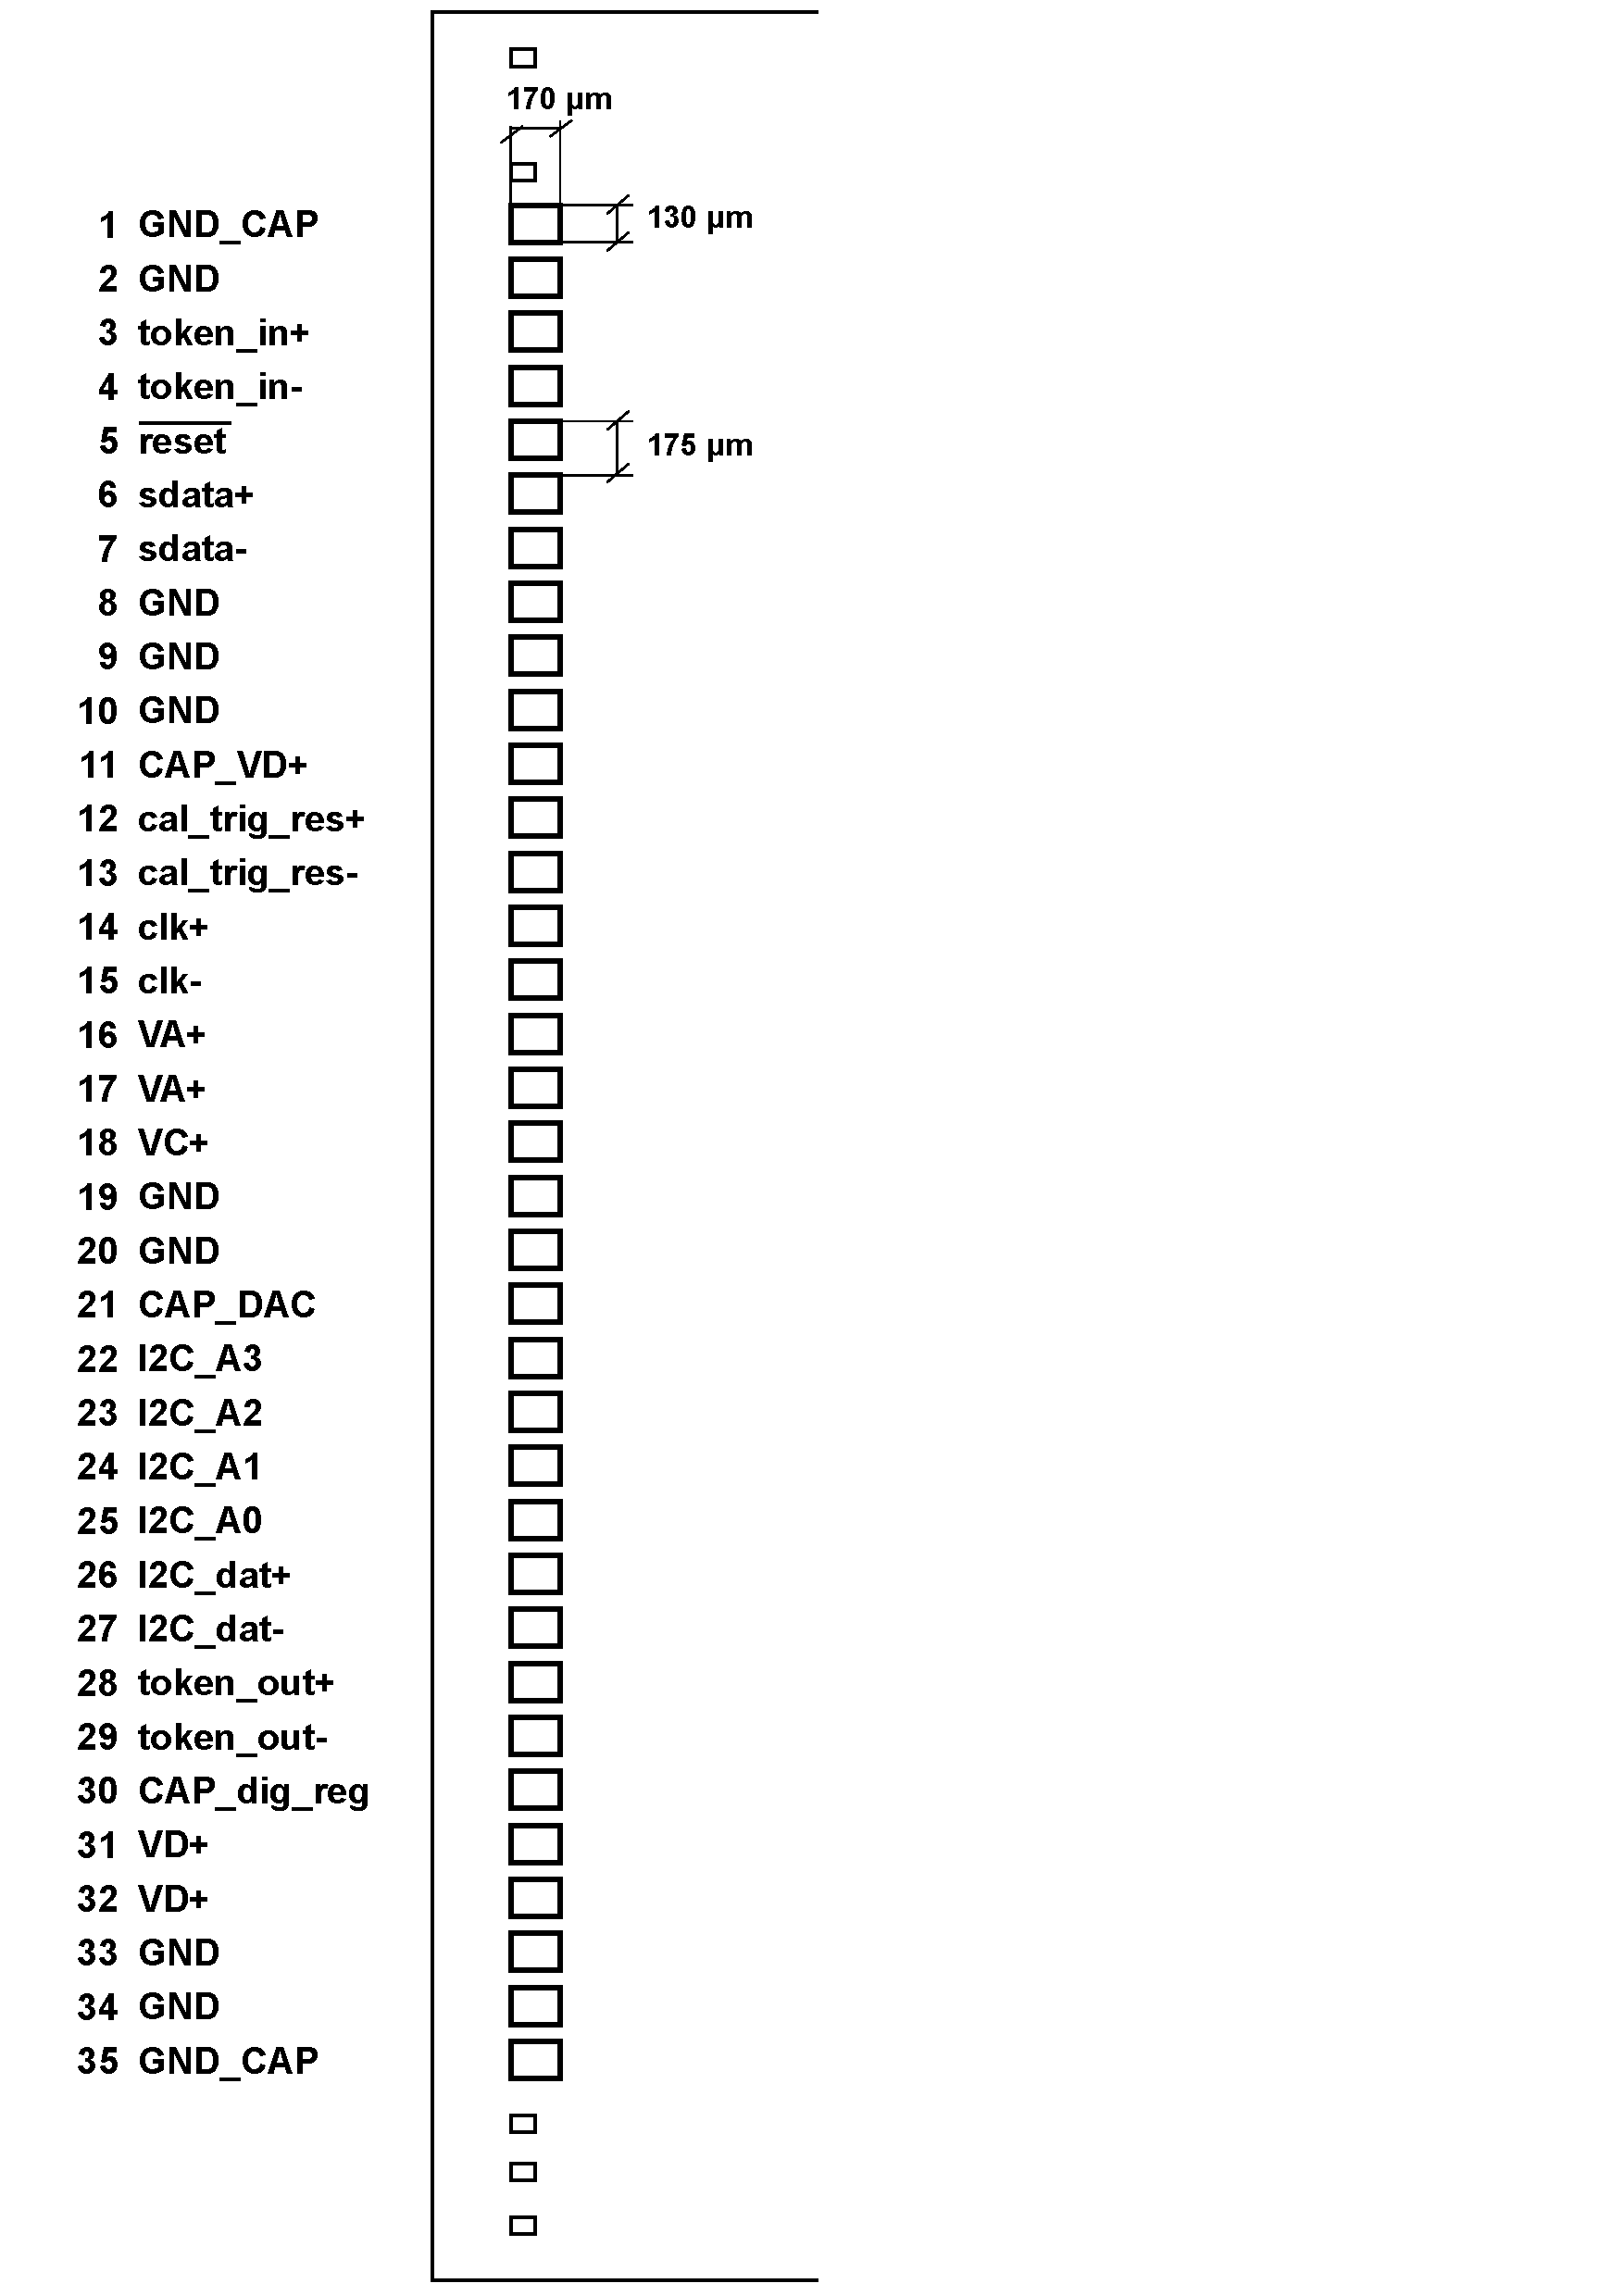
\includegraphics[width=0.9\textwidth]{img/PadLayout.pdf}
	\end{center}
	\caption{Location and names of wire-bond pads on the chip. The pitch of the wirebond pads is 175\,$\mu$m.}
	\label{fig:ROCpadschematic}
\end{figure}


%------------------------------------------------------------------------------

\section{Power supplies}
The PSI46digV2.x ROC needs two supply voltages. The first one is used exclusively for the sensitive analog amplifiers of the pixel unit cells and is called VA+. The recommended value is +1.5\,V. It is a constant current terminal with a programmable current range of about 6-40\,mA. The standard value for operation is 24\,mA and has to be programmed with the DAC called Vana.\\
The second supply voltage is called VD+. It powers all other circuits in the ROC through a total of 5 different voltage regulators. This can be seen in some detail in figure~\ref{fig:ROCpowering}.\\  



\begin{figure}[hbtp]
	\begin{center}
	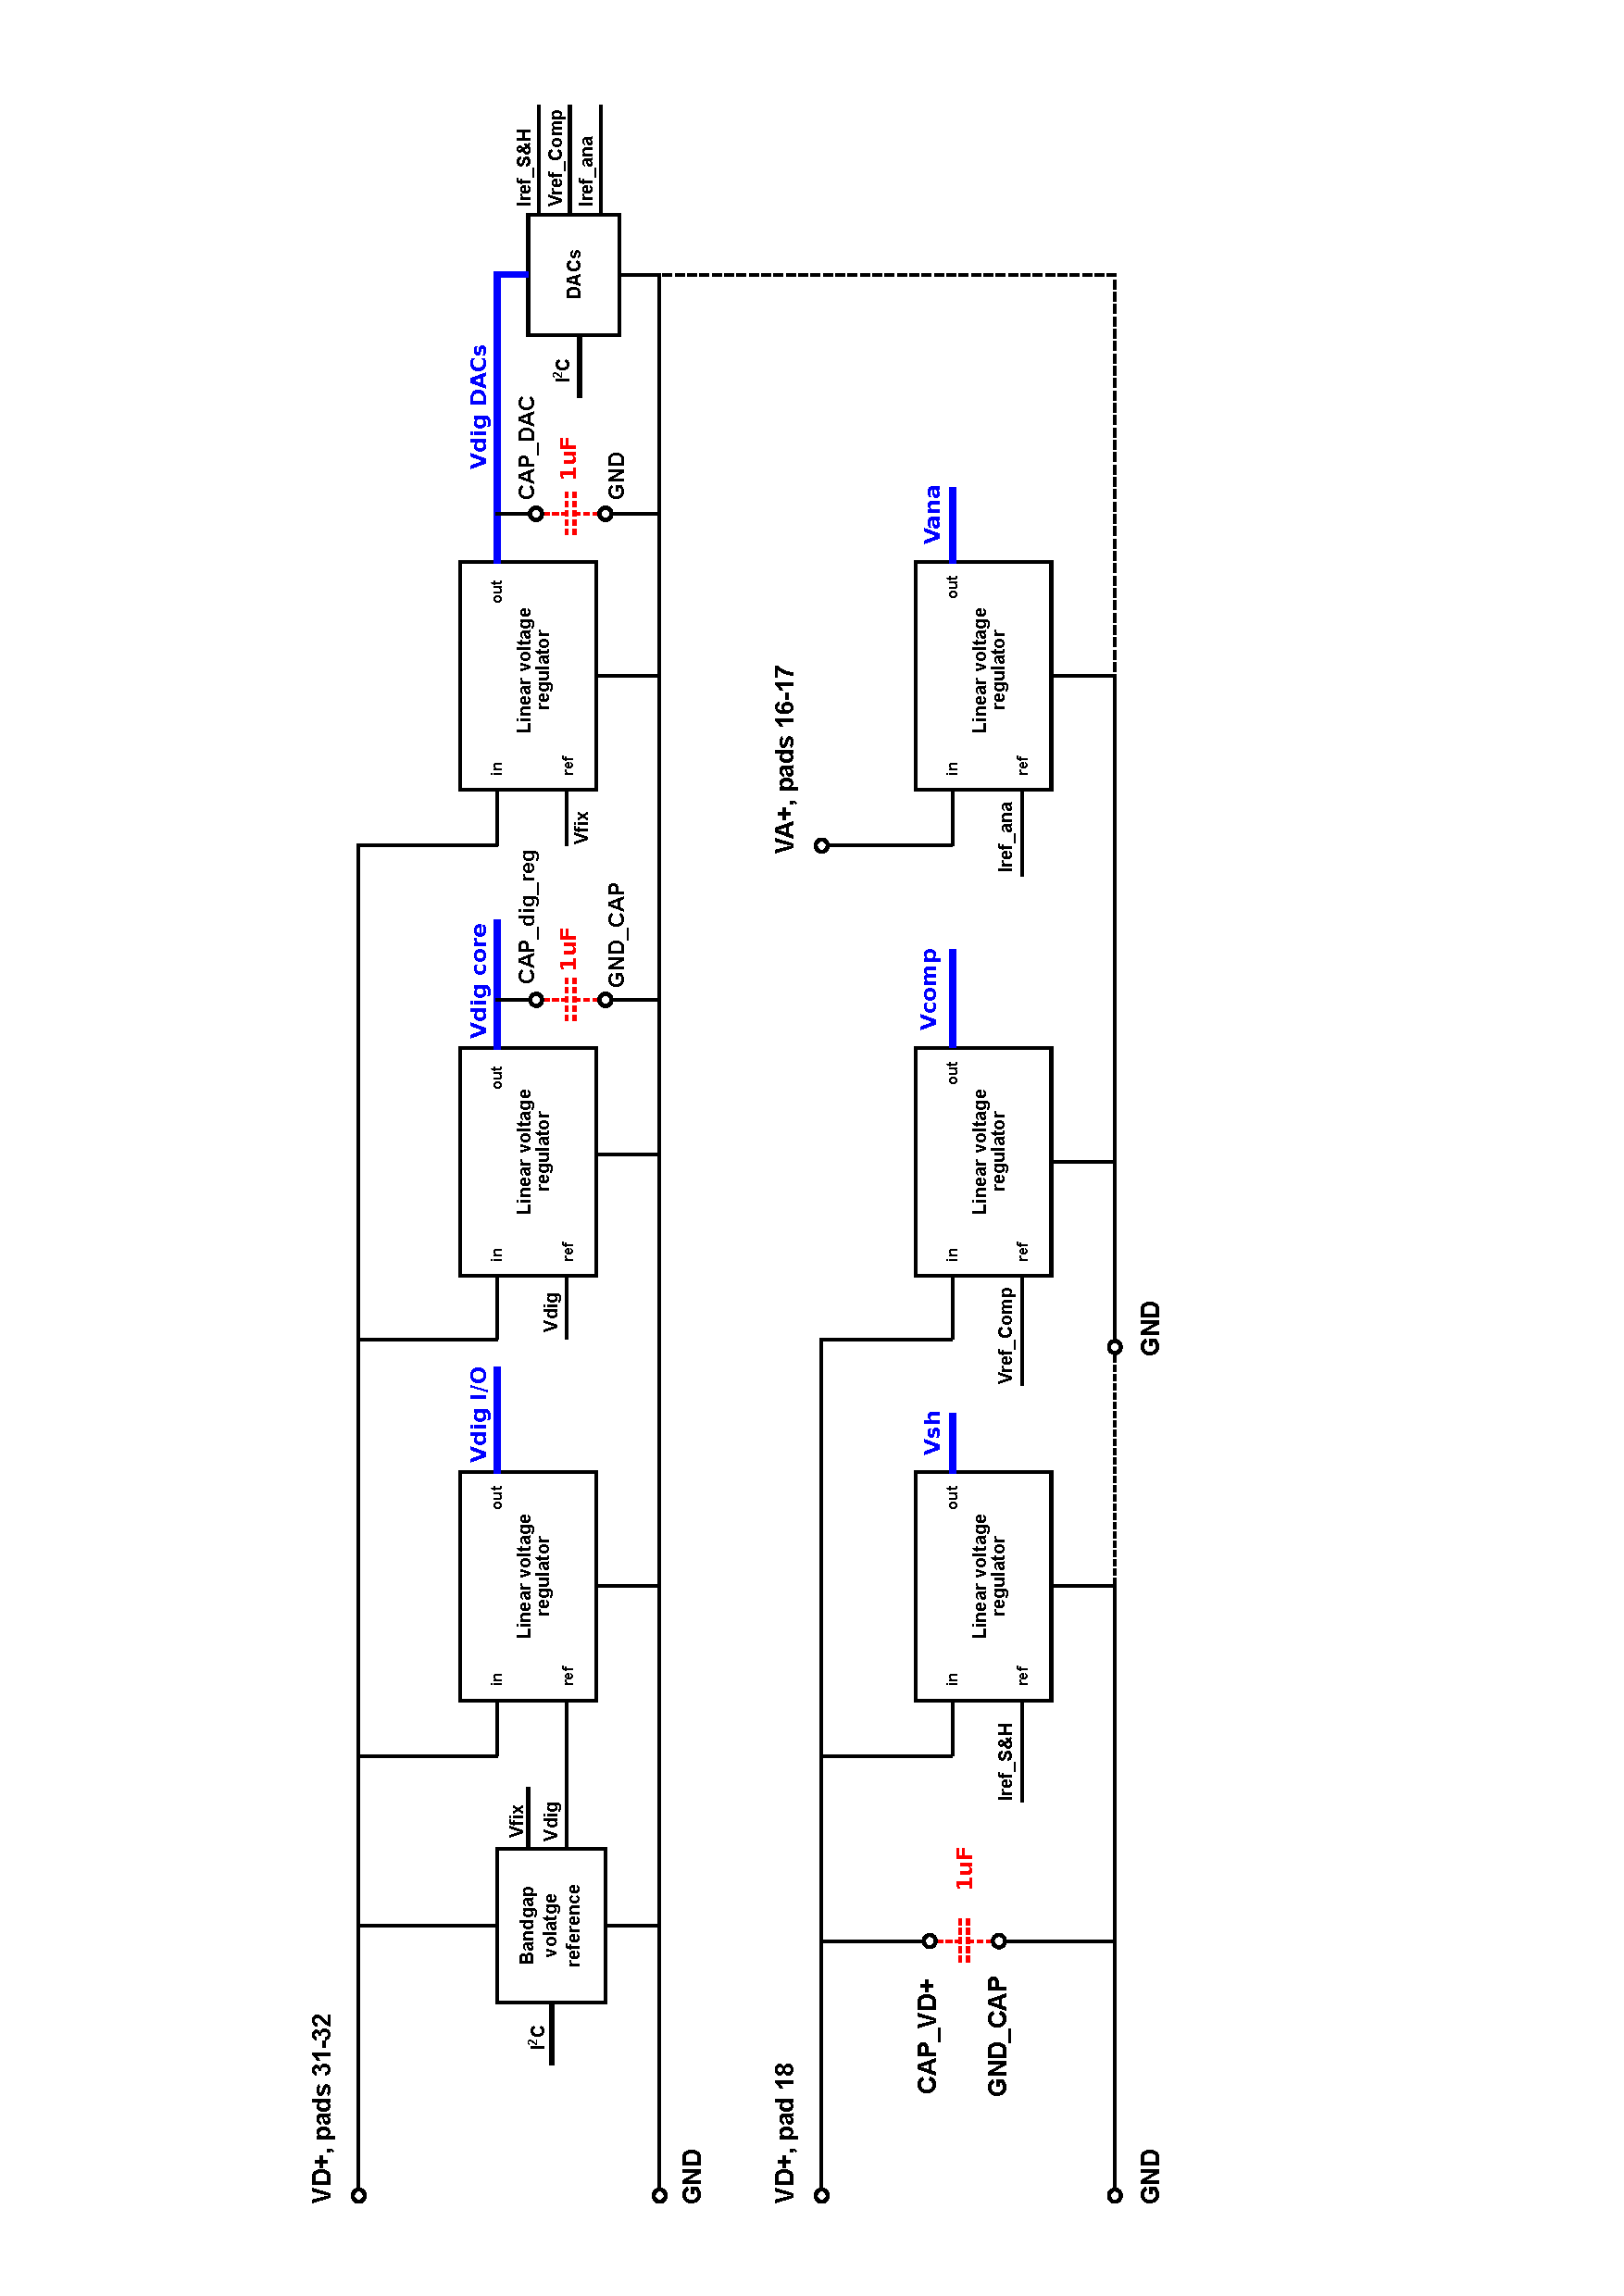
\includegraphics[width=\textwidth]{img/Powering.pdf}
	\end{center}
	\caption{Schematic view of the ROC internal power regulation systems. The red dashed capacitors are external components.}
	\label{fig:ROCpowering}
\end{figure}

\section{Inputs and outputs}
 The ROC has 9 input and 2 output signals. Electrically, there are 3 types of signals: single ended CMOS, custom low voltage differential signals (LVDS) and low current differential signals (LCDS). 
 \subsection{Inputs}
 Single ended signals  are used for slow or static signals. These are the ROC address (I2C\_Ax, pads 22-25) and a hard chip reset signal ($\overline{\mathrm{reset}}$, pad 5). The address bits have internal pull-down resistors connected to GND, while the $\overline{\mathrm{reset}}$ has a pull-up resistor to VD+. The hard reset is a legacy feature and is not needed for proper operation. As it is an active low signal, it can just be left unconnected.\\
The other four inputs are LVDS signals. These are the 40\,MHz clock (clk$\pm$, pads 14-15), a combined calibrate, trigger and reset signal (cal\_trig\_res$\pm$, pads 12-13), the I$^2$C bus data line (I2C\_dat$\pm$, pads 26-27) and the readout token input (token\_in$\pm$, pads 3-4).\\
\subsection{Outputs}
The PSI46digV2.x ROC has two differential output signals. The readout token (token\_out$\pm$, pads 28-29) is a LVDS signal, while the 160\,MBit/sec serial data output (sdata$\pm$, pads 6-7) is a low current differential signal (LCDS).\\
\subsection{Physical signal specification}
The nominal levels for the single ended CMOS inputs are $V_{IL}=0$\,V for logic low and $V_{IH}=$VD+ for logic high. Permitted levels are $V_{IL}<0.5$\,V and $V_{IH}>1.5$\,V. The address input pads can draw up to 150(25)\,$\mu$A in the high(low) state. The current for the $\overline{\mathrm{reset}}$ signal is <5\,$\mu$A.\\ 
For fast signals between ROCs or ROC and TBM at short distances a low voltage differential signalling (LVDS) has been chosen. In order to be more power efficient the ANSI/TIA/EIA standard has been given up. The transmitter is a differential voltage source. The logic levels are $V_{OL}=1.05$\,V and $V_{OL}=1.25$\,V. This gives a nominal differential signal of 200\,mV at a common mode voltage of $V_{CM}=1.15$\,V. No termination is needed for traces up to a length of about 10\,cm. Transmission of up to 1\,m is possible when terminated with the proper cable impedance. Note however, that the signal levels will eventually become very small. The receiver operates with an input voltage difference>50\,mV and a common mode in a wide range between 0.5\,V and Vdig I/O. The later is the regulated I/O power supply (see fig~\ref{fig:ROCpowering}) and can be programmed through the DAC called Vdig in a range between 1.8 and 2.4\,V.\\
The 160\,MBit/sec serial data output (sdata$\pm$) is a low current differential signal (LCDS). The sender is a 1\,mA current switching circuit. The full current is switched to one pad or the other with no current flowing into the second pad. Termination to GND is required at the receiver end. The TBM as the receiver has built in termination resistors of 62\,$\Omega$.\\
All I/O pads have ESD protection diodes to GND and VD+. 
